\documentclass[a4paper,11pt]{scrartcl}

\usepackage{biblatex}
\usepackage{lmodern}
\usepackage[T1]{fontenc}
\usepackage[a4paper, total={14cm, 24cm}]{geometry}
\usepackage{textcomp}
\usepackage{gensymb}
\usepackage{graphicx}
\usepackage{float}
\usepackage{caption}
\usepackage{hyperref}
\usepackage{paralist}
\usepackage{xcolor}
\usepackage{subcaption}
\usepackage[font={footnotesize,it}]{caption}
\usepackage{amsmath,amssymb,amsthm} 
\usepackage{url}
\usepackage{xspace}
\usepackage{algorithmic}
\usepackage{mathpazo}
\usepackage{booktabs}
\usepackage{subfiles}
\usepackage{silence}

% [Settings]

\WarningFilter{DuplicateLabels}

\newcommand{\ie}{ie}
\newcommand{\eg}{eg}
\newcommand{\reffig}[1]{Figure~\ref{#1}}
\newcommand{\refsec}[1]{Section~\ref{#1}}

\setcapindent{1em} %-- for captions of Figures
\setlength\parskip{1em plus 0.1em minus 0.2em}
\setlength\parindent{0pt}
\sffamily

\renewcommand{\algorithmicrequire}{\textbf{Input:}}
\renewcommand{\algorithmicensure}{\textbf{Output:}}

\addbibresource{ref.bib}

% [Title Page] (could be split away)

\titlehead{\centering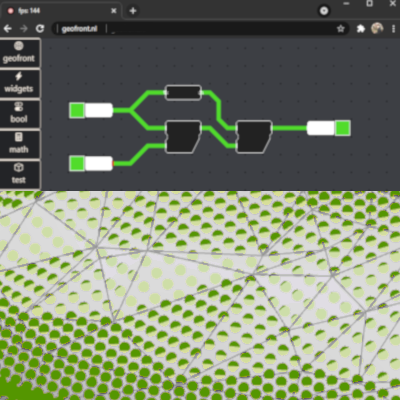
\includegraphics[width=12cm]{images/thumbnail.png}}
\title{Geofront: Browser-based geodata processing using CGAL, GDAL and WebAssembly}

\author{
  Jos Feenstra\\
  student \#4465768 \\
  \url{me@josfeenstra.nl}\\
  \\
  1st supervisor: Stelios Vitalis \\
  2nd supervisor: Ken Arroyo Ohori \\
}

\date{November, 2021}

\begin{document}

\clearpage\maketitle
\thispagestyle{empty}
\sffamily

\begin{center}
  \textbf{Key words:} Geomatics, WebAssembly, 3D geometry, Geodata, Visual programming, 
\end{center}

% [Table of Content] 
\newpage
\tableofcontents

% [Content]
\newpage
\WarningFilter{DuplicateLabels}

%-------------------------------------------------------------------------------------------------%
% An introduction in which the relevance of the project and its place in the 
% context of geomatics is described, along with a clearly-defined problem statement.
\section{Introduction}

% 1. geodata processing is important 
% 2. vpl's makes geodata processing debugable and more insightful. 
% 3. BUT current VPL's lack certain aspects
% 4. use FAIR paradigm to criticize current VPL's 
% 5. go from this to research question

% [JF]: This is super nice, By 'improving a VPL' I dont have to go all 'use case testing' and make a case for a vpl, 
% because I can just state in this introduction "they are useful, look, multiple people are working on them"


\subsection{"making the Case"}

\subsubsection{Findable}
la la la 

\subsubsection{Accessible}
Most vpl's are not 


\subsubsection{Interoperable}
la la la 

\subsubsection{Reusable}
reusability is arguably the main reason why code is important: a structured way of defining a process. 
This way the process itself can be taken and used in different contexts.
vpl's are often not reusable in the same way as code. they are strongly tied to their host environments

%-------------------------------------------------------------------------------------------------%
% A related work section in which the relevant literature is presented and 
% linked to the project. 
% It should show that you clearly know the problem you plan to solve, 
% and that you master the related work. 
\section{Related work}

% ------ research -----

% products 
\subsection{Geomatics tools using WebAssembly}

% 
\subsection{Visual programming languages used within the field of geomatics}

%-------------------------------------------------------------------------------------------------%
% The research questions are clearly defined, along with the scope (ie what you will not be doing).
% To help you define a "good" research question, 
% read \url{https://sites.duke.edu/urgws/files/2014/02/Research-Questions_WS-handout.pdf}.
\section{Research questions}

% ----
\subsection{Sub Questions}



%-------------------------------------------------------------------------------------------------%
% This is not an official section, but important nonetheless
\section{Motivation}



%-------------------------------------------------------------------------------------------------%
% Overview of the methodology to be used.
\section{Methodology}


%-------------------------------------------------------------------------------------------------%
% Having a Gantt chart is probably a better idea then just a list.
\section{Time planning}


%-------------------------------------------------------------------------------------------------%
% Since specific data and tools have to be used, it’s good to present these concretely, 
% so that the mentors know that you have a grasp of all aspects of the project.
\section{Tools and datasets used}



% [Appendix]
\newpage
\printbibliography

\end{document}